% Created 2017-05-15 Mon 12:44
% Intended LaTeX compiler: pdflatex
\documentclass[presentation,10pt]{beamer}
\usepackage[utf8]{inputenc}
\usepackage[T1]{fontenc}
\usepackage{graphicx}
\usepackage{grffile}
\usepackage{longtable}
\usepackage{wrapfig}
\usepackage{rotating}
\usepackage[normalem]{ulem}
\usepackage{amsmath}
\usepackage{textcomp}
\usepackage{amssymb}
\usepackage{capt-of}
\usepackage{hyperref}
\usepackage{amsthm}
\usepackage{amsmath}
\usepackage{amssymb}
\usepackage{mathtools}
\newtheorem{mydef}{Definition}
\newtheorem{mythm}{Theorem}
\newcommand{\dx}{\mathrm{d}}
\newcommand{\var}{\mathrm{Var}}
\newcommand{\cov}{\mathrm{Cov}}
\newcommand{\corr}{\mathrm{corr}}
\newcommand{\pr}{\mathrm{Pr}}
\newcommand{\rarrowd}[1]{\xrightarrow{\text{ \textit #1 }}}
\DeclareMathOperator*{\plim}{plim}
\newcommand{\plimn}{\plim_{n \rightarrow \infty}}
\usepackage{booktabs}
\usepackage{color}
\usepackage{caption}
\usepackage{subcaption}
\def\mathbi#1{\textbf{\em #1}}
\setlength{\parskip}{1em}
\newcommand{\undersetdisp}[2]{\underset{\displaystyle #1}{#2}}
\usetheme{CambridgeUS}
\usecolortheme{beaver}
\author{Zheng Tian}
\date{}
\title{Lecture 3: The GARCH Model}
\hypersetup{
 pdfauthor={Zheng Tian},
 pdftitle={Lecture 3: The GARCH Model},
 pdfkeywords={},
 pdfsubject={},
 pdfcreator={Emacs 25.1.1 (Org mode 9.0.3)}, 
 pdflang={English}}
\begin{document}

\maketitle
\begin{frame}{Outline}
\tableofcontents
\end{frame}



\section{The Problem of ARCH Models}
\label{sec:org432edfa}

\begin{frame}[label={sec:orgf3a2198}]{The problem of ARCH models}
\begin{block}{The principle of parsimony}
\begin{itemize}
\item Merriam-Webster:
\begin{enumerate}
\item the quality of being careful with money or resources
\item the quality or state of being stingy
\end{enumerate}

\item Econometric modeling
\begin{itemize}
\item Use a concise model specification
\item Object to overparameterization
\end{itemize}
\end{itemize}
\end{block}

\begin{block}{The problem of ARCH model}
\begin{itemize}
\item Estimate so many parameters to fully capture higher-order
autoregressive relationship in \(a^2_t\).

\item Think of how many parameters in an ARCH(m) model?
\end{itemize}
\end{block}
\end{frame}


\section{What is the GARCH Model?}
\label{sec:org357ca55}

\begin{frame}[label={sec:orgbf7fd8b}]{The GARCH model}
\begin{block}{Generalized ARCH model}
\begin{itemize}
\item Bollerslev (1986) proposes an extension of ARCH, known as the
Generalized ARCH (GARCH) model.

\item A high-order ARCH model may have a more parsimonious GARCH
representation.
\end{itemize}
\end{block}

\begin{block}{The mean equation}
\[ r_t = \mu_t + a_t \]
where 
\begin{itemize}
\item \(\mu_t\) is modeled with an appropriate regression model or some
ARMA specification.
\item \(a_t\) is the innovation at time \(t\).
\end{itemize}
\end{block}

\begin{block}{The volatility equation}
\[ \sigma^2_t = \var(\alpha^2_t | F_{t-1}) \]
\end{block}
\end{frame}

\begin{frame}[label={sec:org8d57190}]{The GARCH(m, s) model}
\begin{equation}
\label{eq:garchms}
a_t = \sigma_t \epsilon_t,\; \sigma^2_t = \alpha_0 + \sum_{i=1}^m \alpha_i a^2_{t-i} + \sum_{j=1}^s \beta_j \sigma^2_{t-j}
\end{equation}
where
\begin{itemize}
\item \(\epsilon_t \sim i.i.d.(0, 1)\) is a white noise process
\item \(\alpha_0 > 0\), \(\alpha_i \geq 0\) (at least one \(\alpha_i > 0\)),
\(\beta_j \geq 0\)
\item \(\sum_{i=1}^{\mathrm{max}(m,s)}(\alpha_i + \beta_i) < 1\), in which \(\alpha_i
  = 0\) for \(i > m\) and \(\beta_i = 0\) for \(j > s\).
\end{itemize}
\end{frame}

\begin{frame}[label={sec:org443c470}]{ARCH and GARCH model}
\begin{block}{When \(\beta_j = 0\) for all \(j = 1, \ldots, s\)}
\[ GARCH(m, s) \Rightarrow ARCH(m) \]
\end{block}

\begin{block}{GARCH v.s. ARCH and AR v.s. ARMA}
\begin{itemize}
\item An ARCH model can be considered as an AR process of \(a^2_t\).
\item A GARCH model can be considered as an ARMA process of \(a^2_t\).
\item That is why we can write a higher-order ARCH(m) process with a
\emph{parsimonious} GARCH(1, 1) process. 
\begin{itemize}
\item What is the AR representation of ARMA?
\end{itemize}
\end{itemize}
\end{block}
\end{frame}
\begin{frame}[label={sec:org67c6125}]{ARMA representation of GARCH}
\begin{itemize}
\item Let \(\eta_t = \alpha^2_t - \sigma^2_t\).

\item \(E(\eta_t) = 0\), \(\cov(\eta_t, \eta_{t-i}) = 0\) for \(i \geq 1\), but
usually \(\eta_t\) is not i.i.d.

\item A GARCH(m, s) model can be written as
\begin{equation*}
a^2_t = \alpha_0 + \sum_{i=1}^{\mathrm{max}(m, s)} (\alpha_i + \beta_i) a^2_{t-i} + \eta_t - \sum_{j=1}^s \beta_j \eta_{t-j}
\end{equation*}
which can be regarded as an ARMA form for the squared series
\(a^2_t\).

\item For stationarity of \(a^2_t\), we must require that the characteristic
roots of the above ARMA representation lie within the unit circle.
\end{itemize}
\end{frame}


\section{Properties of GARCH(1, 1)}
\label{sec:org0171ce2}

\begin{frame}[label={sec:orgce32aa7}]{The Properties of GARCH(1, 1)}
Consider a GARCH(1, 1)
\[ \sigma^2_t = \alpha_0 + \alpha_1 a^2_{t-1} + \beta_1 \sigma^2_{t-1} \]
where 
$$\alpha_0 > 0, 0 < \alpha_1 \leq 1, 0 \leq \beta_1 \leq 1,
\text{ and } \alpha_1 + \beta_1 < 1$$

\begin{block}{The mean of \(a_t\)}
\begin{itemize}
\item The unconditional mean: \(E(a_t) = E(\sigma_t \epsilon_t) = E(\sigma_t) E(\epsilon_t) = 0\)

\item The conditional mean: \(E_{t-1}(a_t) = \sigma_t E_{t-1}(\epsilon_t) = \sigma_t
  E(\epsilon_t) = 0\)
\end{itemize}
\end{block}
\end{frame}

\begin{frame}[label={sec:orgde6a070}]{The variance of \(\epsilon_t\)}
\begin{block}{The conditional variance}
$$E_{t-1}(a^2_t) = \sigma^2_t = \alpha_0 + \alpha_1 \alpha^2_{t-1} +
\beta_1 \sigma^2_{t-1}$$
\end{block}

\begin{block}{The unconditional variance}
\begin{align*}
& \alpha^2_t = \epsilon^2_t (\alpha_0 + \alpha_1 \alpha^2_{t-1} +
\beta_1 \sigma^2_{t-1}) \\
\Rightarrow & E(a^2_t) = E(\epsilon^2_t) \left[\alpha_0 + \alpha_1 E(a^2_{t-1}) +
\beta_1 E(\sigma^2_{t-1}) \right] \\
\Rightarrow & E(a^2_t) = \alpha_0 + (\alpha_1 + \beta_1) E(a^2_{t-1}) 
\end{align*}

Let \(E(a^2_t) = E(a^2_{t-1})\). We have
\[ E(a^2_t) = \frac{\alpha_0}{1 - \alpha_1 - \beta_1} \]

For the variance must be positive, we require \(\alpha_1 + \beta_1 <
1\). 
\end{block}
\end{frame}

\begin{frame}[label={sec:org35bb86c}]{The variance of \(\epsilon_t\) (cont'd)}
From the ARMA representation of a GARCH(m, s) model
\begin{equation*}
a^2_t = \alpha_0 + 
\sum_{i=1}^{\mathrm{max}(m,s)}(\alpha_i + \beta_i) a^2_{t-i} + \eta_t - \sum_{j=1}^s \beta_j \eta_{t-j}
\end{equation*}
we can also derive the unconditional variance of a stationary \(a_t^2\) series
is 
\begin{equation*}
E(a^2_t) = \frac{\alpha_0}{1-\sum_{i=1}^{\mathrm{max}(m,s)}(\alpha_i + \beta_i)}
\end{equation*}
in which we must require \(\sum_{i=1}^{\mathrm{max}(m,s)}(\alpha_i +
\beta_i) <1\). 
\end{frame}

\begin{frame}[label={sec:orgcde542a}]{The autocorrelation and kurtosis}
\begin{block}{The autocorrelation function}
$$E(a_t a_{t-i}) = E(\sigma_t \epsilon_t \sigma_{t-i} \epsilon_{t-i})
= 0$$
\end{block}

\begin{block}{The kurtosis}
Assume that \(\epsilon_t \sim N(0, 1)\). Given that \(1 - (\alpha_1 +
\beta_1)^2 - 2\alpha^2_1 > 0\), the kurtosis of \(a_t\) is
\begin{equation*}
\frac{3[1 - (\alpha_1 + \beta_1)^2]}{1 - (\alpha_1 + \beta_1)^2 - 2\alpha^2_1} > 3
\end{equation*}
That is, the tail distribution of a GARCH(1, 1) process is heavier
than that of a normal distribution. 
\end{block}
\end{frame}

\begin{frame}[label={sec:orgb1d02ae}]{Volatility persistence}
The roles of \(\alpha_1\) and \(\beta_1\) in volatility persistence are different
\begin{itemize}
\item The larger is \(\alpha_1\), the larger is the response of \(\sigma^2_t\)
to new information. 
\[\text{A shock of } \epsilon_t \rightarrow a_t \rightarrow
  \sigma^2_{t+1} \]

\item The larger is \(\beta_1\), the more persistence is the conditional
variance. 
\[\text{A shock of } \epsilon_t \rightarrow a_t \rightarrow
  \sigma^2_{t+1} \rightarrow \sigma^2_{t+2} \]
\end{itemize}
\end{frame}

\begin{frame}[label={sec:org1f8eba7}]{Volatility persistence}
Consider two GARCH(1, 1) models
\begin{gather*}
\sigma^2_t = 1 + 0.6 a^2_{t-1} + 0.2 \sigma^2_{t-1} \\
\sigma^2_t = 1 + 0.2 a^2_{t-1} + 0.6 \sigma^2_{t-1}
\end{gather*}
\begin{figure}[htbp]
\centering
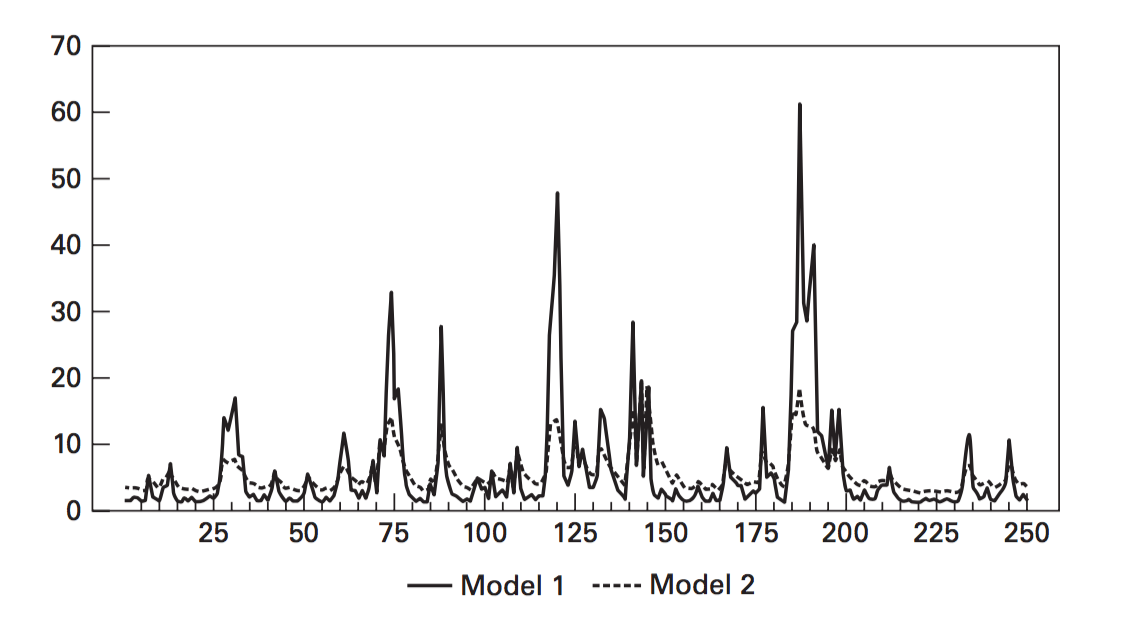
\includegraphics[width=0.9\textwidth,height=0.6\textheight]{img/volatile_persist.png}
\end{figure}
\end{frame}


\section{Estimation and forecasting}
\label{sec:orgb368a05}

\begin{frame}[label={sec:orgc25a44b}]{Maximum likelihood estimation}
The conditional log-likelihood function is similar to that of ARCH model
\begin{equation}
\label{eq:arch-logL}
\ell(\boldsymbol{\alpha}, \boldsymbol{\beta} | a_1, \ldots, a_T) = 
\sum_{t=1}^T \left[ -\frac{1}{2} \ln(2\pi) - \frac{1}{2} \ln(\sigma^2_t) - \frac{1}{2} \frac{a^2_t}{\sigma^2_t}  \right]
\end{equation}

The difference is that now \(\sigma^2_t\) is a GARCH model
\[\sigma^2_t = \alpha_0 + \sum_{i=1}^m \alpha_i a^2_{t-i} +
\sum_{j=1}^s \beta_j \sigma^2_{t-j} \]
\end{frame}

\begin{frame}[label={sec:orgc47dced}]{Check model adequacy}
\begin{block}{Compute the standardized residuals}
\[ \tilde{a}_t = \frac{\hat{a}_t}{\hat{\sigma}_t} \]
\end{block}

\begin{block}{Check the mean equation}
Use the Ljung-Box statistic for \{\(\tilde{a}_t\)\}.
\end{block}

\begin{block}{Check the volatility equation}
Use the Ljung-Box statistic for \{\(\tilde{a}_t\)\}.
\end{block}
\end{frame}

\begin{frame}[label={sec:org4c50b83}]{Model diagnosis}
\begin{block}{Goodness of fit}
\begin{itemize}
\item SSR. Since \(\epsilon_t = a^2_t / \sigma^2_t\), we can compute SSR as
\[ SSR = \sum_{t=1}^T \frac{\hat{a}^2_t}{\hat{\sigma}^2_t} \]

\item The log-likelihood function. 

\[2\ell = \sum_{t=1}^T \left[ \ln(\hat{\sigma}^2_t) + \frac{\hat{a}^2_t}{\hat{\sigma}^2_t}
  \right] - T\ln(2\pi) \]
\end{itemize}
\end{block}

\begin{block}{Information criteria}
\begin{itemize}
\item \(AIC = -2\ell + 2n\)
\item \(BIC = -2\ell + n \ln(T)\)
\end{itemize}
\end{block}
\end{frame}



\begin{frame}[label={sec:orgf602572}]{Forecasting}
\begin{block}{1-step-ahead forecast}
\begin{equation*}
\sigma^2_h(1) = \alpha_0 + \alpha_1 a^2_h + \beta_1 \sigma^2_h
\end{equation*}
\end{block}

\begin{block}{2-step-ahead forecast}
\begin{equation}
\begin{split}
\sigma^2_{h+2} &= \alpha_0 + \alpha_1 a^2_{h+1} + \beta_1 \sigma^2_{h+1} \\
&= \alpha_0 + (\alpha_1 + \beta_1) \sigma^2_{h+1} + \alpha_1 \sigma^2_{h+1}(\epsilon^2_{h+1}-1)
\end{split}
\end{equation}

Given that \(E(\epsilon^2_{h+1} - 1 | F_h) = 0\), the 2-step-ahead
forecast is
\[ \sigma^2_h(2) = \alpha_0 + (\alpha_1 + \beta_1)\sigma^2_h(1) \]
\end{block}
\end{frame}

\begin{frame}[label={sec:org6741465}]{Forecasting (cont'd)}
\begin{block}{The \(\ell\)-step-ahead forecast}
\[ \sigma^2_h(\ell) = \alpha_0 + (\alpha_1 +
\beta_1)\sigma^2_h(\ell-1), \text{ for } \ell > 1 \]
\end{block}

\begin{block}{As \(\ell \rightarrow \infty\)}
\begin{equation*}
\sigma^2(\ell) =
\frac{\alpha_0\left[1-(\alpha_1+\beta_1)^{\ell-1}\right]}{1-\alpha_1-\beta_1}
+ (\alpha_1+\beta_1)^{\ell-1}\sigma^2_h(1)
\end{equation*}
Therefore,
\begin{equation*}
\sigma^2(\ell) \rightarrow \frac{\alpha_0}{1-\alpha_1-\beta_1}, \text{ as } \ell\rightarrow\infty
\end{equation*}
provided that \(\alpha_1+\beta_1<1\). 
\end{block}
\end{frame}
\end{document}